\documentclass{article}%
\usepackage[T1]{fontenc}%
\usepackage[utf8]{inputenc}%
\usepackage{lmodern}%
\usepackage{textcomp}%
\usepackage{lastpage}%
\usepackage[head=40pt,margin=0.5in,bottom=0.6in]{geometry}%
\usepackage{graphicx}%
%
\title{\textbf{ONU nombra a Eduardo Stein como representante para la crisis migratoria venezolana}}%
\author{EFE}%
\date{19/09/2018}%
%
\begin{document}%
\normalsize%
\maketitle%
\textbf{URL: }%
http://www.eluniversal.com/politica/21100/onu{-}nombra{-}a{-}eduardo{-}stein{-}como{-}representante{-}para{-}la{-}crisis{-}migratoria{-}venezolana\newline%
%
\textbf{Periodico: }%
EU, %
ID: %
21100, %
Seccion: %
politica\newline%
%
\textbf{Palabras Claves: }%
NO\_TIENE\newline%
%
\textbf{Derecho: }%
5, %
Otros Derechos: %
1.10, %
Sub Derechos: %
1.10.1\newline%
%
\textbf{EP: }%
NO\newline%
\newline%
%
\textbf{\textit{El exvicepresidente de Guatemala "trabajará para promover el diálogo y el consenso necesarios para la respuesta humanitaria" en Venezuela}}%
\newline%
\newline%
%
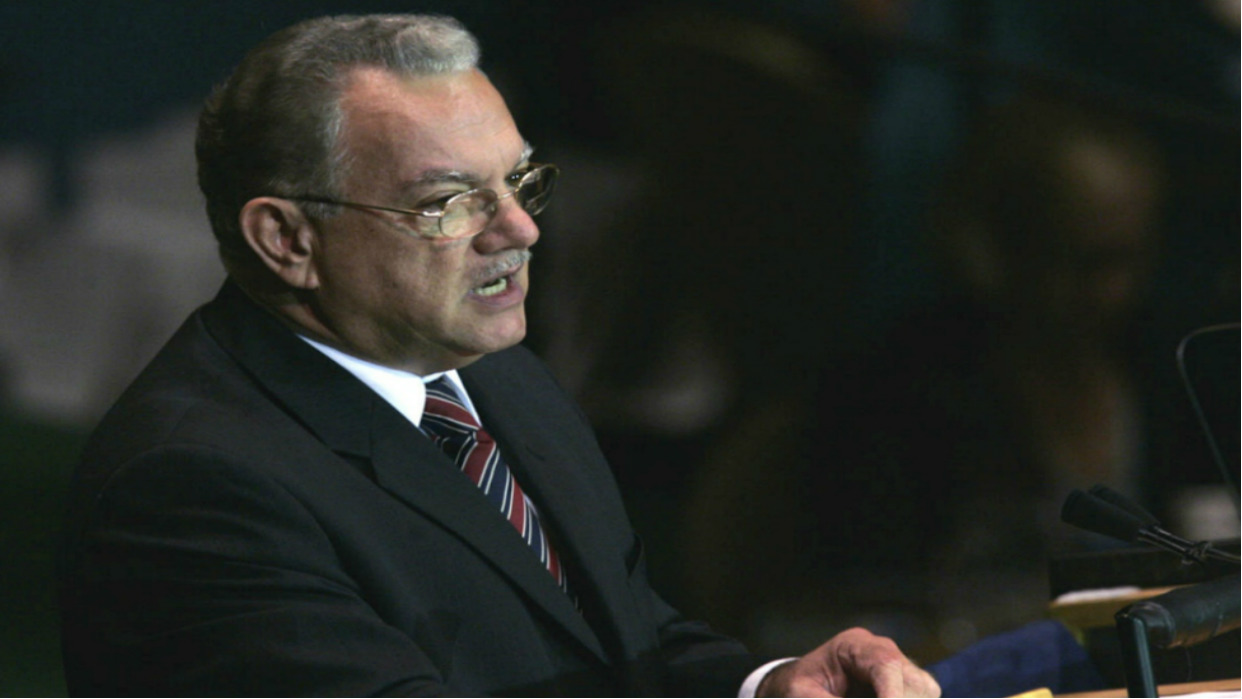
\includegraphics[width=300px]{122.jpg}%
\newline%
%
Ginebra.{-}El exvicepresidente de Guatemala, Eduardo Stein, fue nombrado este miércoles representante especial de la Organización de las Naciones Unidas (ONU) para los refugiados y migrantes de Venezuela.%
\newline%
%
Eduardo Stein "trabajará para promover el diálogo y el consenso necesarios para la respuesta humanitaria, incluyendo el acceso a territorio, protección de los refugiados, estatuto regular, y la identificación de soluciones para refugiados y migrantes venezolanos", señalaron en un comunicado conjunto la Agencia de la ONU para los Refugiados (Acnur) y la Organización Internacional para las Migraciones (OIM).%
\newline%
%
El exvicepresidente guatemalteco (quien ocupó el cargo entre 2004 y 2008) "promoverá un enfoque regional coherente y armonizado de cara a la situación de Venezuela en coordinación con los gobiernos nacionales, las organizaciones internacionales y otros actores relevantes", según explica el texto.%
\newline%
%
El nombramiento llega dos días después de que el canciller colombiano, Carlos Holmes Trujillo, pidiera en Ginebra la creación de "un fondo humanitario de emergencia para fortalecer la capacidad presupuestal a fin de hacerle frente" a la crisis política y económica en Venezuela, reseñó Efe.%
\newline%
%
El titular de Relaciones Exteriores colombiano señaló también "la necesidad de la designación de un alto funcionario dentro del marco de Naciones Unidas, cuya tarea sea coordinar la acción multilateral.~Cuanto más pronto mejor, porque la crisis aumenta de una manera dramática día a día", dijo Trujillo el lunes ante la prensa, tras reunirse con la alta comisionada de la ONU para los Derechos Humanos, Michelle Bachelet.%
\newline%
%
Colombia, que comparte 2.200 kilómetros de la frontera con Venezuela, ya había advertido en las últimas semanas que no tenía capacidad para enfrentar en solitario la llegada de migrantes venezolanos, que superó el millón de personas en los últimos años, de los que 820.000 regularizaron su situación.%
\newline%
%
"Yo me temo que esa cifra es mayor y nos preocupa muchísimo la tendencia que están presentando esas cifras, porque de seguir como van estaríamos hablando de cerca de 4 millones de Venezolanos al final de este año fuera de su país", alertó Trujillo.%
\newline%
%
\end{document}